% Options for packages loaded elsewhere
\PassOptionsToPackage{unicode}{hyperref}
\PassOptionsToPackage{hyphens}{url}
\PassOptionsToPackage{dvipsnames,svgnames,x11names}{xcolor}
%
\documentclass[
  letterpaper,
  DIV=11,
  numbers=noendperiod]{scrreport}

\usepackage{amsmath,amssymb}
\usepackage{lmodern}
\usepackage{iftex}
\ifPDFTeX
  \usepackage[T1]{fontenc}
  \usepackage[utf8]{inputenc}
  \usepackage{textcomp} % provide euro and other symbols
\else % if luatex or xetex
  \usepackage{unicode-math}
  \defaultfontfeatures{Scale=MatchLowercase}
  \defaultfontfeatures[\rmfamily]{Ligatures=TeX,Scale=1}
\fi
% Use upquote if available, for straight quotes in verbatim environments
\IfFileExists{upquote.sty}{\usepackage{upquote}}{}
\IfFileExists{microtype.sty}{% use microtype if available
  \usepackage[]{microtype}
  \UseMicrotypeSet[protrusion]{basicmath} % disable protrusion for tt fonts
}{}
\makeatletter
\@ifundefined{KOMAClassName}{% if non-KOMA class
  \IfFileExists{parskip.sty}{%
    \usepackage{parskip}
  }{% else
    \setlength{\parindent}{0pt}
    \setlength{\parskip}{6pt plus 2pt minus 1pt}}
}{% if KOMA class
  \KOMAoptions{parskip=half}}
\makeatother
\usepackage{xcolor}
\setlength{\emergencystretch}{3em} % prevent overfull lines
\setcounter{secnumdepth}{5}
% Make \paragraph and \subparagraph free-standing
\ifx\paragraph\undefined\else
  \let\oldparagraph\paragraph
  \renewcommand{\paragraph}[1]{\oldparagraph{#1}\mbox{}}
\fi
\ifx\subparagraph\undefined\else
  \let\oldsubparagraph\subparagraph
  \renewcommand{\subparagraph}[1]{\oldsubparagraph{#1}\mbox{}}
\fi


\providecommand{\tightlist}{%
  \setlength{\itemsep}{0pt}\setlength{\parskip}{0pt}}\usepackage{longtable,booktabs,array}
\usepackage{calc} % for calculating minipage widths
% Correct order of tables after \paragraph or \subparagraph
\usepackage{etoolbox}
\makeatletter
\patchcmd\longtable{\par}{\if@noskipsec\mbox{}\fi\par}{}{}
\makeatother
% Allow footnotes in longtable head/foot
\IfFileExists{footnotehyper.sty}{\usepackage{footnotehyper}}{\usepackage{footnote}}
\makesavenoteenv{longtable}
\usepackage{graphicx}
\makeatletter
\def\maxwidth{\ifdim\Gin@nat@width>\linewidth\linewidth\else\Gin@nat@width\fi}
\def\maxheight{\ifdim\Gin@nat@height>\textheight\textheight\else\Gin@nat@height\fi}
\makeatother
% Scale images if necessary, so that they will not overflow the page
% margins by default, and it is still possible to overwrite the defaults
% using explicit options in \includegraphics[width, height, ...]{}
\setkeys{Gin}{width=\maxwidth,height=\maxheight,keepaspectratio}
% Set default figure placement to htbp
\makeatletter
\def\fps@figure{htbp}
\makeatother

\KOMAoption{captions}{tableheading}
\makeatletter
\makeatother
\makeatletter
\@ifpackageloaded{bookmark}{}{\usepackage{bookmark}}
\makeatother
\makeatletter
\@ifpackageloaded{caption}{}{\usepackage{caption}}
\AtBeginDocument{%
\ifdefined\contentsname
  \renewcommand*\contentsname{Table of contents}
\else
  \newcommand\contentsname{Table of contents}
\fi
\ifdefined\listfigurename
  \renewcommand*\listfigurename{List of Figures}
\else
  \newcommand\listfigurename{List of Figures}
\fi
\ifdefined\listtablename
  \renewcommand*\listtablename{List of Tables}
\else
  \newcommand\listtablename{List of Tables}
\fi
\ifdefined\figurename
  \renewcommand*\figurename{Figure}
\else
  \newcommand\figurename{Figure}
\fi
\ifdefined\tablename
  \renewcommand*\tablename{Table}
\else
  \newcommand\tablename{Table}
\fi
}
\@ifpackageloaded{float}{}{\usepackage{float}}
\floatstyle{ruled}
\@ifundefined{c@chapter}{\newfloat{codelisting}{h}{lop}}{\newfloat{codelisting}{h}{lop}[chapter]}
\floatname{codelisting}{Listing}
\newcommand*\listoflistings{\listof{codelisting}{List of Listings}}
\makeatother
\makeatletter
\@ifpackageloaded{caption}{}{\usepackage{caption}}
\@ifpackageloaded{subcaption}{}{\usepackage{subcaption}}
\makeatother
\makeatletter
\@ifpackageloaded{tcolorbox}{}{\usepackage[many]{tcolorbox}}
\makeatother
\makeatletter
\@ifundefined{shadecolor}{\definecolor{shadecolor}{rgb}{.97, .97, .97}}
\makeatother
\makeatletter
\makeatother
\ifLuaTeX
  \usepackage{selnolig}  % disable illegal ligatures
\fi
\IfFileExists{bookmark.sty}{\usepackage{bookmark}}{\usepackage{hyperref}}
\IfFileExists{xurl.sty}{\usepackage{xurl}}{} % add URL line breaks if available
\urlstyle{same} % disable monospaced font for URLs
\hypersetup{
  pdftitle={Evo Compressor},
  pdfauthor={FLUX:: Immersive},
  colorlinks=true,
  linkcolor={blue},
  filecolor={Maroon},
  citecolor={Blue},
  urlcolor={Blue},
  pdfcreator={LaTeX via pandoc}}

\title{Evo Compressor}
\author{FLUX:: Immersive}
\date{2/6/23}

\begin{document}
\maketitle
\ifdefined\Shaded\renewenvironment{Shaded}{\begin{tcolorbox}[boxrule=0pt, breakable, frame hidden, enhanced, sharp corners, interior hidden, borderline west={3pt}{0pt}{shadecolor}]}{\end{tcolorbox}}\fi

\renewcommand*\contentsname{Table of contents}
{
\hypersetup{linkcolor=}
\setcounter{tocdepth}{2}
\tableofcontents
}
\bookmarksetup{startatroot}

\hypertarget{introduction}{%
\chapter{Introduction}\label{introduction}}

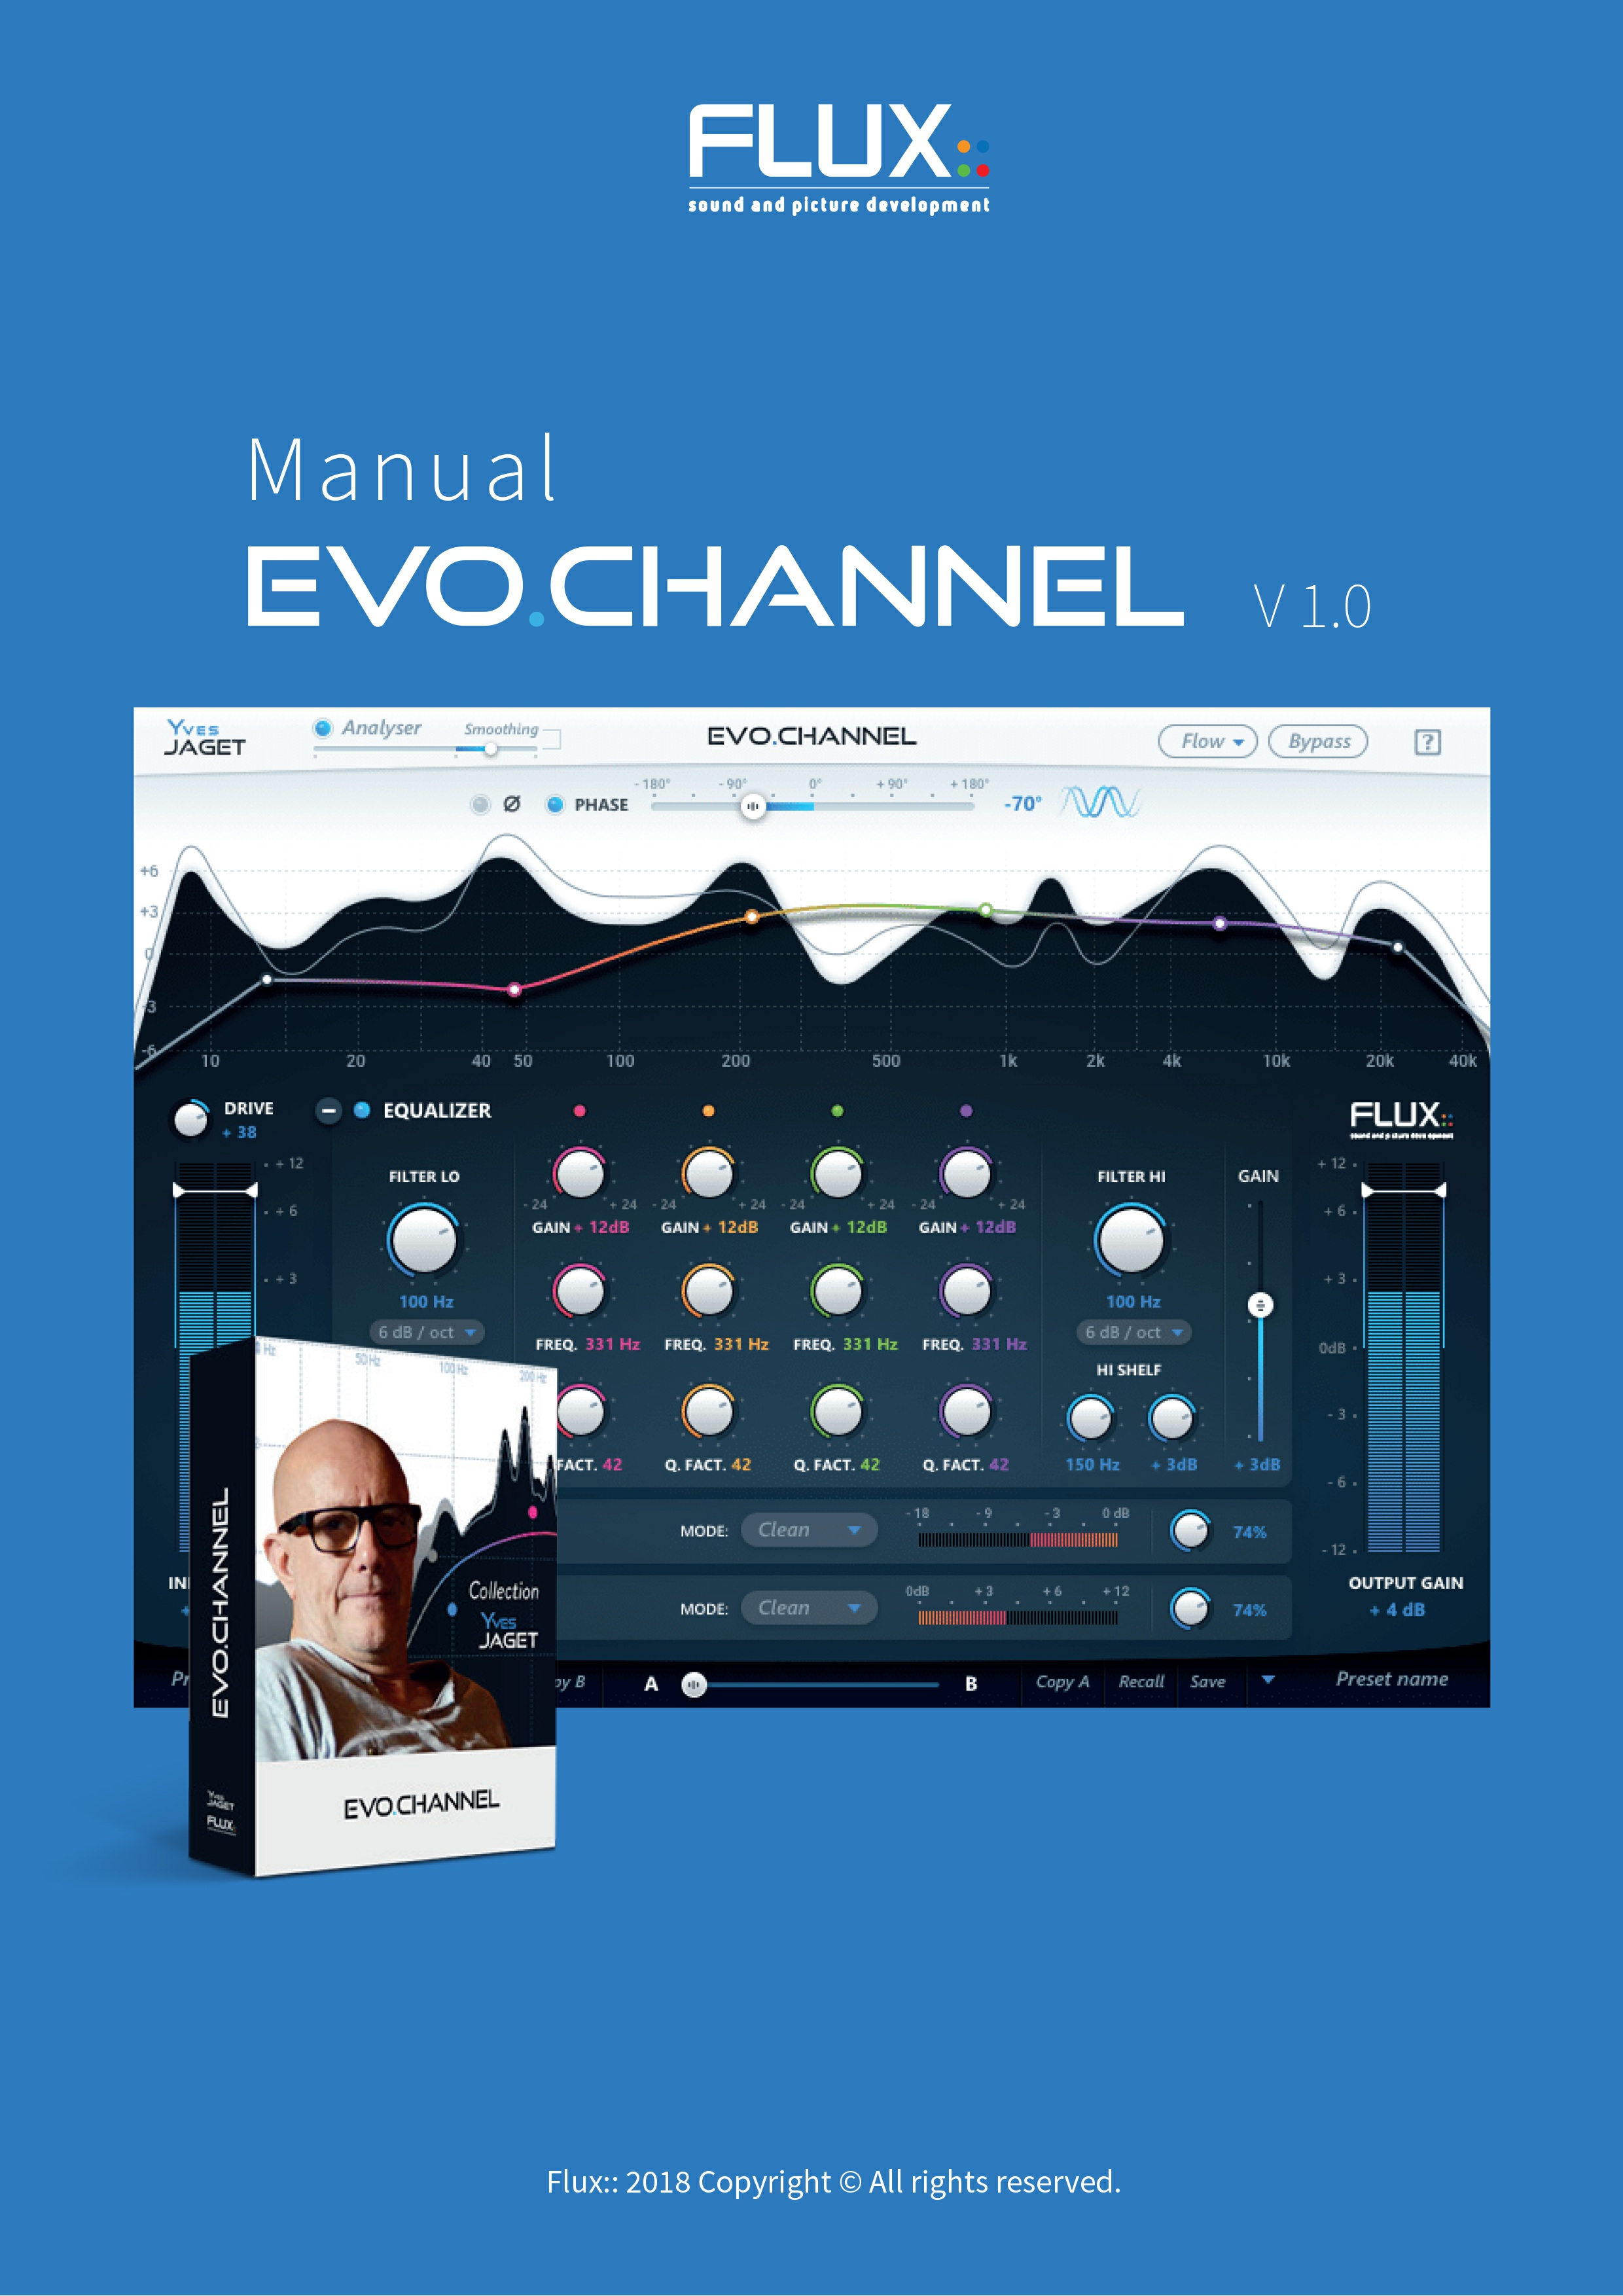
\includegraphics{include/ManualEvoChannel-000.jpg}

\href{https://www.flux.audio/project/evo-series/}{Product Page}
\textbar{}
\href{https://shop.flux.audio/en_US/products/evo-series-pack}{Shop Page}

\textbf{EVO Comp - The Sound Attitude Generator}

In addition to controlling the signal dynamics, the compressor is often
used for shaping the attitude of a sound. To use a compressor in a
creative and artistic fashion it's important that it's easy to use and
has the ability to create an interesting sound.

The EVO Channel and EVO Comp compressor offers a wide range and variety
of sound with nine different compression modes, and a Wet / Dry control
for adjusting the level of compression, allowing for parallel
compression within the module.

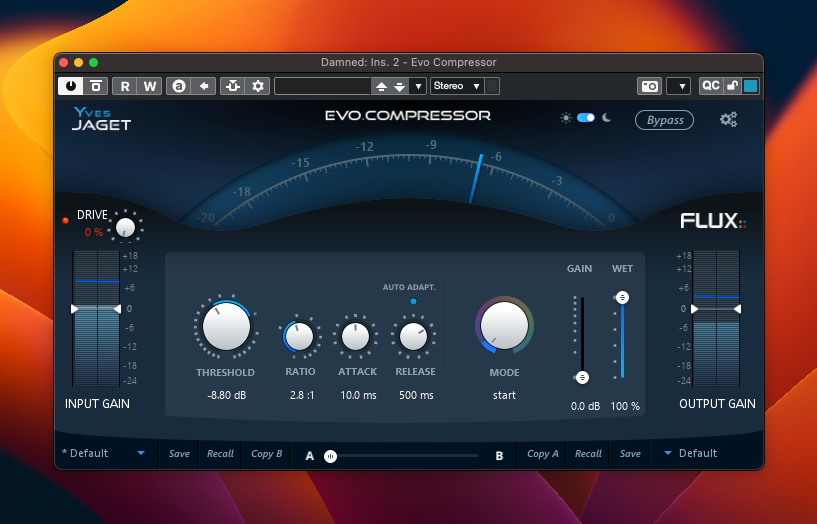
\includegraphics{include/evoComp.png}

\bookmarksetup{startatroot}

\hypertarget{general-settings}{%
\chapter{General Settings}\label{general-settings}}

\hypertarget{bypass}{%
\section{Bypass}\label{bypass}}

Global bypass, when pressed, the signal is routed directly from the
inputs to the outputs.

Value Range : Enabled/Disabled

Default Value : Disabled

\hypertarget{skin}{%
\section{Skin}\label{skin}}

The look of the EVO Comp user interface.

Value Range : Light/Dark

Default Value : Light

\bookmarksetup{startatroot}

\hypertarget{module-settings}{%
\chapter{Module Settings}\label{module-settings}}

\hypertarget{input}{%
\section{Input}\label{input}}

\hypertarget{input-gain}{%
\subsection{Input Gain}\label{input-gain}}

The input gain control trims the level of the signal at the input of EVO
Comp. The meter shows both RMS signal (VU-Meter, blue) and peak signal
(peak meter, green), from -24 to +18 dB range, referenced at -18dB.

Value Range : -24.0 dB / +18.0 dB

Colors : - Blue : RMS Value - Green : Peak Value

Default Value : 0.0 dB

\hypertarget{drive}{%
\subsection{Drive}\label{drive}}

In EVO Comp a signal Drive is available direct at the input Gain for
restoring and maintaining the vitality of the sound.

The drive module has been specially designed to add a soft saturation
and warmth to your audio tracks.

Value Range : 0\% / 100\%

Default Value : 0\%

\hypertarget{compressor}{%
\section{Compressor}\label{compressor}}

In addition to controlling the signal dynamics, the compressor is often
used for shaping the attitude of a sound. To use a compressor in a
creative and artistic fashion it's important that it's easy to use and
has the ability to create an interesting sound.

The EVO Comp's compressor module is based on the Pure Compressor's
dynamics engine, and the same range of compression types are available
in EVO Comp through the different modes available (each mode corresponds
to a fine tuning of Pure Compressor). As some modes use a LID
compression (Level Independent Detection) in parallel, a gain reduction
may be processed even if the audio level is below the threshold.

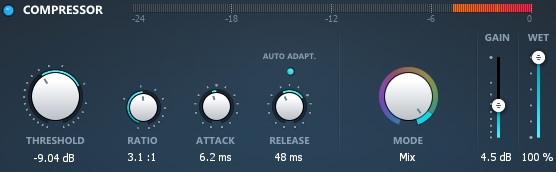
\includegraphics{include/ManualEvoChannel-010.jpg}

\hypertarget{mode}{%
\subsection{Mode}\label{mode}}

The compressor module gives you up to 9 modes of compression.

Available modes :

\begin{itemize}
\tightlist
\item
  Start
\item
  Kick/Snare
\item
  Overhead
\item
  Drum Bus
\item
  Bass
\item
  Acoustic
\item
  Piano
\item
  Vocal
\item
  Mix
\end{itemize}

Default Value : Start

\hypertarget{threshold}{%
\subsection{Threshold}\label{threshold}}

Threshold value of the compressor.

Value Range : -42.0dB / +18.0dB

Default Value : Depends on the Mode.

\hypertarget{ratio}{%
\subsection{Ratio}\label{ratio}}

Compression ratio parameter.

Value Range : 1.0:1 / 10.0:

Default Value : Depends on the Mode.

\hypertarget{attack}{%
\subsection{Attack}\label{attack}}

Attack value of the compressor.

Value Range : 0.1ms / 1000.0ms

Default Value : Depends on the Mode.

\hypertarget{release}{%
\subsection{Release}\label{release}}

Release value of the compressor.

Value Range : 1ms / 10000ms

Default Value : Depends on the Mode.

\hypertarget{auto-adapt.}{%
\subsection{Auto Adapt.}\label{auto-adapt.}}

When enabled, the compressor adapts its release time to the input signal
depending on the audio signal, but won't exceed the release time value.

Value Range : Enabled / Disabled

Default Value : Enabled

\hypertarget{gain-reduction-display}{%
\subsection{Gain Reduction Display}\label{gain-reduction-display}}

Displays the gain reduction performed by the compressor.

Value Range : 0dB / -24dB

\hypertarget{compressor-output-gain}{%
\subsection{Compressor Output Gain}\label{compressor-output-gain}}

Gain stage at the output of the compressor module.

Value Range : 0.0dB / 24.0dB

Default Value : 0.0dB

\hypertarget{wet}{%
\subsection{Wet}\label{wet}}

Wet parameter defines how much of the compressed signal is mixed with
the original signal, for parallel compression.

Value Range : 0\% / 100\%

Default Value : 100\%

\hypertarget{output}{%
\section{Output}\label{output}}

\hypertarget{output-gain}{%
\subsection{Output Gain}\label{output-gain}}

The output gain control trims the level of the signal at the output of
EVO Comp. The meter shows both RMS signal (VU-Meter, blue) and peak
signal (peak meter, green), from -24 to +18 dB range, referenced at
-18dB.

Value Range : -24.0 dB / +18.0 dB

Colors : - Blue : RMS Value - Green : Peak Value

Default Value : 0.0 dB

\bookmarksetup{startatroot}

\hypertarget{geek-settings}{%
\chapter{Geek Settings}\label{geek-settings}}

These settings are available by clicking on the ``Yves Jaget'' icon.

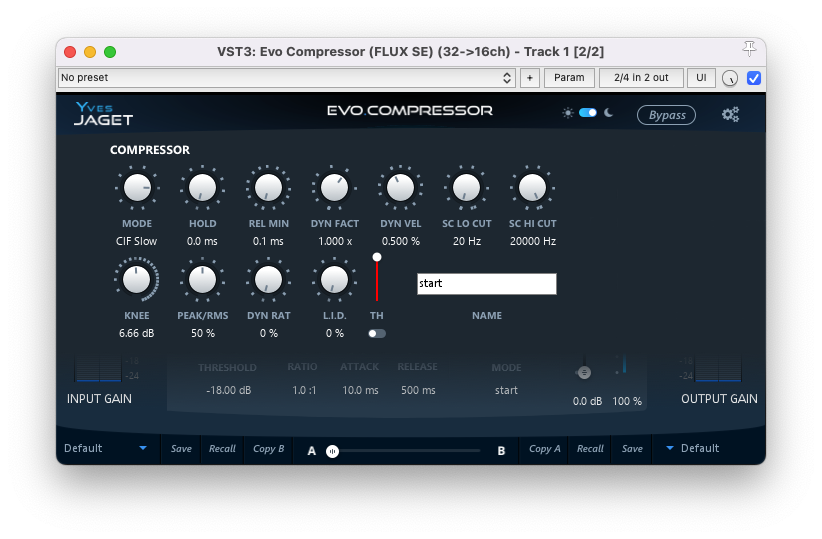
\includegraphics{include/evoComp_geek.png}

\hypertarget{mode-1}{%
\section{Mode}\label{mode-1}}

Default Value: ClF Slow\\
8 different detection modes are available:

\begin{itemize}
\tightlist
\item
  Solera: The Attack setting also controls the integration time for RMS
  detection.
\item
  Solera Feed Backward: The Attack setting also controls the integration
  time for RMS detection which is done on the output of the processor.
  Note also that the Solera Feed Backward prevents to use the external
  side chain because it's the processed signal which feed the side
  chain.
\item
  Classic Fast: The integration time for RMS detection is 10 ms with no
  direct relation with the Attack setting.
\item
  Classic Medium: The integration time for RMS detection is 40 ms with
  no direct relation with the Attack setting.
\item
  Classic Slow: The integration time for RMS detection is 80 ms with no
  direct relation with the Attack setting.
\item
  Classic Feed Backward Fast: The integration time is 10 ms for RMS
  detection which is done on the output of the processor. Note also that
  the Feed Backward mode prevents to use the external side chain because
  it's the processed signal which feed the side chain.
\item
  Classic Feed Backward Medium: The integration time is 40 ms for RMS
  detection which is done on the output of the processor. Note also that
  the Feed Backward mode prevents to use the external side chain because
  it's the processed signal which feed the side chain.
\item
  Classic Feed Backward Slow: The integration time is 80 ms for RMS
  detection which is done on the output of the processor. Note also that
  the Feed Backward mode prevents to use the external side chain because
  it's the processed signal which feed the side chain.
\end{itemize}

\begin{quote}
These Feed Backward modes have been inspired by vintage hardware
architectures. they create a sort of auto regulation of the processing
which produces a naturally beefy sound. The output volume also control
the feedback level.
\end{quote}

\hypertarget{hold}{%
\section{Hold}\label{hold}}

Unit: ms\\
Value Range: 0 ms / 500 ms.\\
Default Value: 0 ms

This parameter is the only one in the time related settings, that is
independent per dynamic processor. The compressor and the expander may
have different hold time.

\begin{quote}
Used in the Expander section, this setting allows very precise gating of
drum tracks. It can also be used for creative purpose on the other
dynamic sections.
\end{quote}

\hypertarget{release-minimum}{%
\section{Release Minimum}\label{release-minimum}}

Unit: ms\\
Value Range: 0.67ms / 5000.00\\
Step: 0.01\\
Default Value: 1.30 ms

Sets the minimum release value when in Advanced Mode.

\hypertarget{dynamic-factor}{%
\section{Dynamic Factor}\label{dynamic-factor}}

Unit: x\\
Value Range: 0 / 3.0\\
Step: variable.\\
Default Value: 1

Amplify or dim the extracted real time dynamic informations.

\hypertarget{dynamic-velocity}{%
\section{Dynamic Velocity}\label{dynamic-velocity}}

Unit: \%\\
Value Range: 10 / 1000\\
Step: 1\\
Default Value: 50 \%

Sets the speed of variation on the dynamic informations.

\hypertarget{sc-lo-cut}{%
\section{SC Lo Cut}\label{sc-lo-cut}}

Unit: Hz\\
Value Range: 20 to 24000 Default Value: 20

Filters out the low-end from the detection circuit.

\hypertarget{sc-hi-cut}{%
\section{SC Hi Cut}\label{sc-hi-cut}}

Unit: Hz\\
Value Range: 20 to 24000 Default Value: 20000

Filters out the high-end from the detection circuit.

\hypertarget{knee}{%
\section{Knee}\label{knee}}

Unit: dB\\
Value Range: 0 to +24\\
Default Value: 0

Sets the smoothness of the transmission curve for the specific dynamic
processing section. The curve is smoothed around the threshold value of
the dB amount set with the knee value.

\hypertarget{peak-detection-amount}{%
\section{Peak Detection Amount}\label{peak-detection-amount}}

Unit: \%\\
Value Range: 0 / 100\\
Step: 1\\
Default Value: 0 \%

Instant peak value can be added to the RMS signal feeding the detector
section, making the dynamic processing more sensitive to audio
transients.

\hypertarget{dynamic-ratio}{%
\section{Dynamic Ratio}\label{dynamic-ratio}}

Unit: \%\\
Value Range: 0 / 100\\
Step: 1\\
Default Value: 0 \%

This setting relaxes the ratio applied to the processor section when the
detected signal dynamic raises.

This setting literally opens the sound, increases the dynamic impression
and keeps some crest by adjusting in real time the ratio of every
dynamic processing section regarding both their current settings about
ratio and the signal content (mainly dynamic range). To start
understanding this setting and easily hear it, take a full mixed drum
kit or a complete mix with punchy drums, set the compression threshold,
ratio to get something near pumping or an aggressive compression.

Then increase the output gain to compensate the gain lost and then
toggle between 0 and 100\% of Dynamic Ratio. At 100 \% you should hear
more air in the sound, more transient and less compression impression;
especially in terms of attack.

\hypertarget{l.i.d..-level-independent-detector}{%
\section{L.I.D.. (Level Independent
Detector)}\label{l.i.d..-level-independent-detector}}

Unit: \%\\
Value Range: 0 / 100\\
Step: 1\\
Default Value: 0 \%

Allows process the audio signal independently of the sound level but
regarding the signal dynamic range. It is mixed with the standard
compression scheme.

\begin{quote}
Take a piece of full mixed music, set the ratio to 3-4 and the
compression will start working. Now set the threshold of the compressor
to the maximum value, the compressor will stop working because the sound
level will never reach the threshold. Then increase the L.I.D.. and you
will see (and hear) the compression working again!!! Now decrease or
increase the input gain (in Solera or before, as you want) and you will
see that the compression will continue to work equally; it's totally,
completely independent of the sound level and depends only on Ratio,
Knee and sound content.

How can this be used? When you have too much dynamic in the sound, going
for e.g.~from -3, -6 dB Vu (or less) to +12 dB; If you want to compress
the low levels you will hear the sound ™pumping∫ when the sound reaches
the High levels and the only thing to do with standard compressor will
be to increase the threshold to rescue some airiness in the sound. But
when doing that the compressor will not work any more on the low levels,
and you will hear some sound differences (in term density, live space,
grain etcº ) especially when the compressor starts working. With Solera
L.I.D.., adjust the threshold and ratio on the High levels to what you
think OK, then increase the L.I.D.. (from 20 to 50 \%) and listen now
the low levels and especially the transition between Low and High
levels. You can also start increasing the ratio to increase the effect.
You'll then notice that the compression will always be active but can
still take care of High, loud levels (unless you set 100\% L.I.D..) and
make the compression very smooth and no more pumping. In addition with
the Dynamic Ratio function, you'll be able to set a constant and very
natural envelop that allows to increase low levels, low frequency and to
keep important transients.
\end{quote}

\hypertarget{l.i.d..-threshold}{%
\section{L.I.D.. Threshold}\label{l.i.d..-threshold}}

Sets the gain range of the L.I.D. parameter.

\begin{itemize}
\tightlist
\item
  Up: Increasing of the L.I.D. action
\item
  Down: Decreasing of the L.I.D. action
\end{itemize}

The current L.I.D. Threshold value is reflected by two blue lines on the
Dynamic Activity display.

For Compressor and DCompressor sections, the L.I.D. action is effective
only when the orange Dynamic Activity (18) exceeds the area between the
two blue lines. For Expander and DExpander sections, the L.I.D. action
is effective only when the orange Dynamic Activity (18) stays inside the
area between the two blue lines.

\hypertarget{l.i.d..-maximum}{%
\section{L.I.D.. Maximum}\label{l.i.d..-maximum}}

When engaged, the threshold for the processing is determined by the
maximum values from RMS/peak detection OR from the signal dynamic
detection. The L.I.D. Threshold is still active, but the L.I.D. mix
button is disabled.

\begin{quote}
This feature allows the whole process to be more reactive to the signal
content. It worth to be tried on drum tracks.
\end{quote}

\bookmarksetup{startatroot}

\hypertarget{shortcuts}{%
\chapter{Shortcuts}\label{shortcuts}}

Shortcuts have been added to further enhance the user interaction and
improve the workflow.

\begin{longtable}[]{@{}
  >{\raggedright\arraybackslash}p{(\columnwidth - 2\tabcolsep) * \real{0.5000}}
  >{\raggedright\arraybackslash}p{(\columnwidth - 2\tabcolsep) * \real{0.5000}}@{}}
\toprule()
\begin{minipage}[b]{\linewidth}\raggedright
Shortcut
\end{minipage} & \begin{minipage}[b]{\linewidth}\raggedright
Description
\end{minipage} \\
\midrule()
\endhead
Mouse Click + Alt + Shift & Reset all compressor parameters to the
default value of the Mode \\
\bottomrule()
\end{longtable}

\bookmarksetup{startatroot}

\hypertarget{plugin-settings}{%
\chapter{Plugin Settings}\label{plugin-settings}}

Clicking the cogwheel symbol opens a window with a range of general
settings and a direct access button to the user manual.

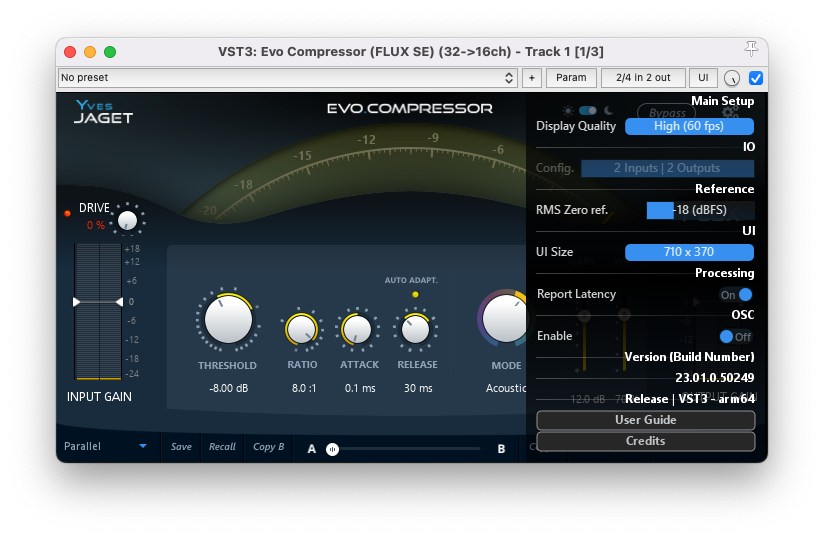
\includegraphics{include/evoComp_opt.png}

\hypertarget{main-setup}{%
\section{Main Setup}\label{main-setup}}

\hypertarget{ui-refresh-rate}{%
\subsection{UI Refresh Rate}\label{ui-refresh-rate}}

Max refresh rate of the plug-in's UI.

\hypertarget{io}{%
\section{I/O}\label{io}}

\hypertarget{input-output}{%
\subsection{Input / Output}\label{input-output}}

I/O Config and Layout is not always available, though it is always
displayed, it can only be edited in some configurations and formats.

\hypertarget{config}{%
\subsection{Config}\label{config}}

Current I/O configuration, is only available in certain VST hosts;
typically hosts with limited capabilities for handling multichannel
configurations.

\hypertarget{layout}{%
\subsection{Layout}\label{layout}}

Available I/O routings based on current I/O configuration. Layout is
available for editing if more than two input channels are available. If
the Layout is changed from the default value, an asterisk * is displayed
next to the Layout information in the Input section.

\hypertarget{processing}{%
\section{Processing}\label{processing}}

\hypertarget{report-latency}{%
\subsection{Report Latency}\label{report-latency}}

Enables/Disables the latency reporting to the host.

\hypertarget{automation}{%
\section{Automation}\label{automation}}

\hypertarget{multithread}{%
\subsection{Multithread}\label{multithread}}

Enables/Disables Multithread Automation.

\hypertarget{osc}{%
\section{OSC}\label{osc}}

OSC is available in EVO Comp.

\hypertarget{enable}{%
\subsection{Enable}\label{enable}}

Enables/Disables OSC control and mapping of the plug-in's parameters.

\hypertarget{version-information}{%
\section{Version Information}\label{version-information}}

Plug-in version and build-number information.

\hypertarget{user-manual-credits}{%
\section{User Manual / Credits}\label{user-manual-credits}}

Quick link to the User Manual. Plug-in creation credits.

\bookmarksetup{startatroot}

\hypertarget{preset-management}{%
\chapter{Preset Management}\label{preset-management}}

EVO Comp, as well as all other FLUX:: plug-ins, provides two preset
slots referred to as slot A and slot B, which provide access to two sets
of parameter settings simultaneously. In addition to just recall the
settings for each of the slots individually and alternate between their
settings, a morphing slider is provided offering the possibility to
morph between the slots and their corresponding settings. When clicking
on one of the preset slots, the built in preset manager appears.


\includegraphics{include/ManualEvoChannel-013.png}

\hypertarget{preset-sections}{%
\section{Preset Sections}\label{preset-sections}}

EVO Comp provides two preset sections referred to as section A and
section B, offering simultaneous access to two full sets of parameter
settings. Clicking the A section (bottom left) or the B section (bottom
right), or clicking the arrow in the Current Selected Preset display,
opens a new window accessing the built-in preset manager.

\hypertarget{save}{%
\section{Save}\label{save}}

Save replaces the selected preset by a new one under the same name
featuring the current settings. If you want to keep an existing preset
without your new modifications, just select an empty place into the
preset list, enter a new name for this modified preset featuring the
current settings and press Save. Recall

Once a preset is selected from the preset list it must be explicitly
loaded into section A or the section B by using the recall button. A
preset is effective only after it has been recalled.

\hypertarget{copy-a-copy-b}{%
\section{Copy A / Copy B}\label{copy-a-copy-b}}

The current parameters of a section are copied to the other one. The
section A or B is re-initialized with the current values and the
morphing slider is parked at 100\% of the corresponding section.

\hypertarget{morphing-slider}{%
\section{Morphing Slider}\label{morphing-slider}}

Morphs the parameter values of both parameter sections, it has no unity
or specific value display; it provides morphing of the current values
from both of the parameter sections (A \& B). A double-click on one side
of the slider area toggles between the two parameter sections. The
actual result of the morphed parameter settings can be saved as a new
preset.

\bookmarksetup{startatroot}

\hypertarget{preset-manager}{%
\chapter{Preset Manager}\label{preset-manager}}

The preset manager contains two preset banks, the Factory bank contains
factory presets, this bank is not available for saving of presets but
any of the presets can be loaded into a preset slot and then saved into,
the User bank, where all user presets are saved.

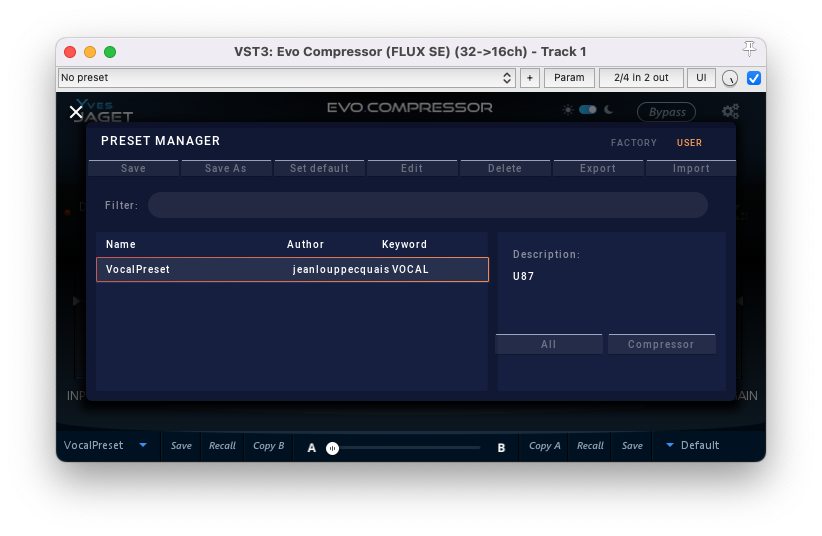
\includegraphics{include/evoComp_userpreset.png}

In the preset manager, any preset can be loaded into a preset slot by
double clicking on the name of the desired preset in the actual preset
list, the preset will then be loaded into the preset slot corresponding
to the position of the morphing slider.

\begin{itemize}
\tightlist
\item
  Additional controls in the preset manager
\item
  Recall A loads the selected preset into the corresponding slot.
\item
  Recall B loads the selected preset into the corresponding slot.
\item
  Update, saves the current settings into the selected preset.
  (Available in User Bank only)
\item
  New, saves the current settings into a new preset. (Available in User
  Bank only)
\item
  Duplicate creates a copy of the selected preset and saves it to the
  list.
\item
  Edit allows for changes to the preset meta properties. (Available in
  User Bank only)
\item
  Delete, removes the selected preset. (Available in User Bank only)
\item
  Export, creates a file reflecting the content of the current preset
  bank.
\item
  Import, allows for import of a preset bank file by adding the imported
  banks content to the content in the current preset bank.
\end{itemize}

When saving or editing a preset, an option to protect the preset is
presented. The preset protection, if engaged, only allows the original
preset author to uncheck and edit the preset. This means that you can
protect your presets in a multi-user configuration. Protected presets
can only be modified using the session used for their creation. If used
in another user session they can only be imported or deleted.

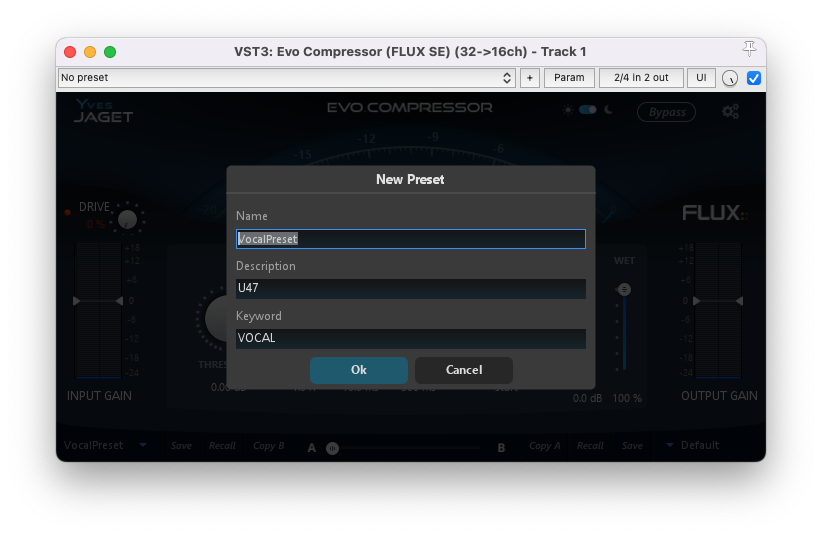
\includegraphics{include/evoComp_preset2.png}
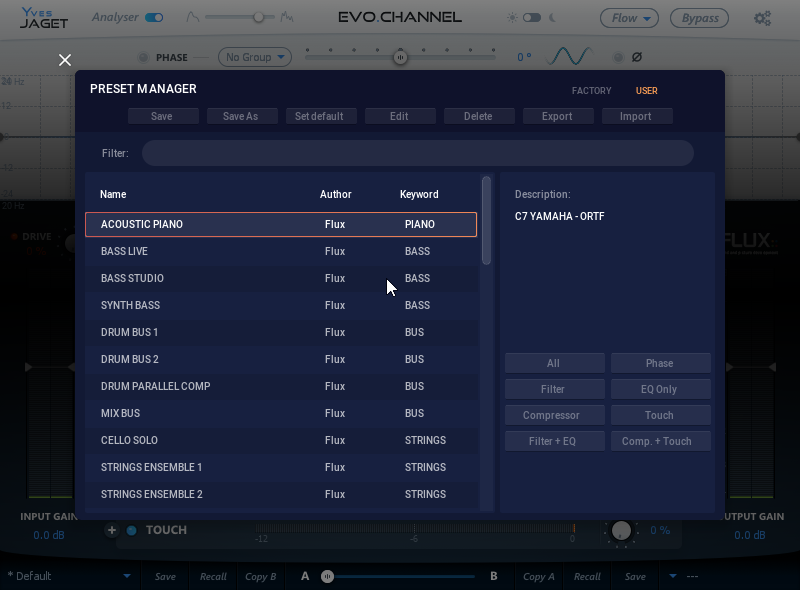
\includegraphics{include/ManualEvoChannel-014.png}

\bookmarksetup{startatroot}

\hypertarget{specifications}{%
\chapter{Specifications}\label{specifications}}

\hypertarget{availability}{%
\section{Availability}\label{availability}}

EVO Comp is available in:

AU / VST / VST3 / AAX Native\emph{/ AAX AudioSuite} / Waves WPAPI

* \emph{AAX Native \& AAX AudioSuite in Pro Tools 11 and later}

\hypertarget{processing-1}{%
\section{Processing}\label{processing-1}}

EVO Comp provides :

\begin{itemize}
\tightlist
\item
  Up to 16 channels Input/Output in VST/VST3/AU/AAX.
\item
  Up to 8 channels in WPAPI for Waves Soundgrid.
\item
  64-bits internal floating point processing.
\item
  Sampling rate up to 384 kHz.
\end{itemize}

\hypertarget{hardware-requirements}{%
\section{Hardware Requirements}\label{hardware-requirements}}

A graphic card fully supporting OpenGL 2.0 is required.

\begin{itemize}
\tightlist
\item
  macOS : OpenGL 2.0 required -- Mac Pro 1.1 \& Mac Pro 2.1 are not
  supported.
\item
  Windows : If your computer has an ATi or NVidia graphics card, please
  assure the latest graphic drivers from the ATi or NVidia website are
  installed.
\end{itemize}

\hypertarget{software-license-requirements}{%
\section{Software License
Requirements}\label{software-license-requirements}}

In order to use the software an iLok.com user account is required (the
iLok USB Smart Key is not required).

\hypertarget{compatibility}{%
\section{Compatibility}\label{compatibility}}

All major native formats are supported

\hypertarget{windows-10-in-64-bits-only.}{%
\subsection{Windows -- 10, in 64 bits
only.}\label{windows-10-in-64-bits-only.}}

\begin{itemize}
\tightlist
\item
  VST (2.4)
\item
  VST3 (3.1)
\item
  AAX Native*
\item
  AAX AudioSuite*
\item
  Waves WPAPI
\end{itemize}

\hypertarget{macos-intel-and-arm}{%
\subsection{macOS (Intel and ARM)}\label{macos-intel-and-arm}}

All versions from Sierra (10.12) to latest. (Compatible with previous
versions but not supported)

\begin{itemize}
\tightlist
\item
  VST (2.4)
\item
  VST3 (3.1)
\item
  AU
\item
  AAX Native*
\item
  AAX AudioSuite*
\item
  Waves WPAPI
\end{itemize}

* \emph{AAX Native \& AAX AudioSuite in Pro Tools 11 and later}



\end{document}
